\documentclass[10pt]{article}

\usepackage[utf8]{inputenc}
\usepackage[T2A]{fontenc}
\usepackage[russian, english]{babel}

\usepackage{amssymb, amsmath, textcomp, tabularx, graphicx}
\usepackage{indentfirst}

\title{Отчет по заданию 2}
\author{Андрей Коновалов, 073}
\date{}

\begin{document}

\maketitle

\section{Постановка задачи}

Известна средняя за два года урожайность ячменя пяти разновидностей на каждом из шести полей.
Хочется понять, как отличается урожайность разновидностей ячменя.

\section{Результаты}

Визуализация исходных данных показана на рис. 1 и 2.

\begin{figure}[h]
  \centering
  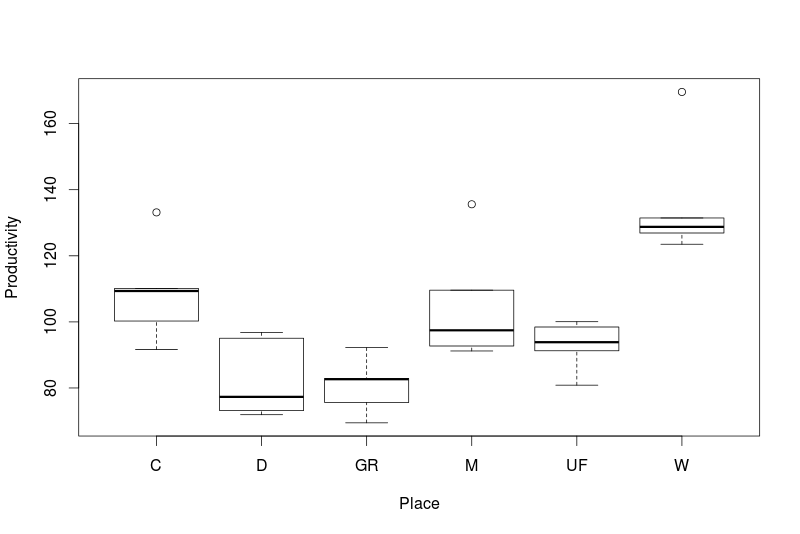
\includegraphics[scale=0.4]{overview_place.png}
  \caption{Boxplot для урожайности и поля.}
\end{figure}

\begin{figure}[h]
  \centering
  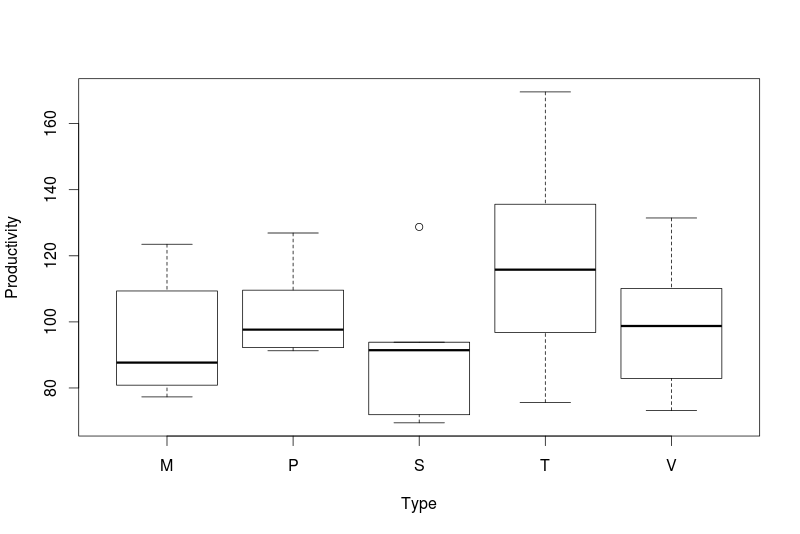
\includegraphics[scale=0.4]{overview_type.png}
  \caption{Boxplot для урожайности и типа ячменя.}
\end{figure}

Для решения задачи используем двухфакторную ANOVA.
Получим следующие значения p-value для факторов: 0.0000005 для поля и 0.0025 для типа ячменя.
Значимыми факторами являются как поле (что вполне ожидаемо, поскольку поля могут быть разными по размеру и вообще между собой не особо связаны), так и тип ячменя.

На рис. 3 изображен QQ-plot, который не показывает существенных отклонений от нормальности.

\begin{figure}[h]
  \centering
  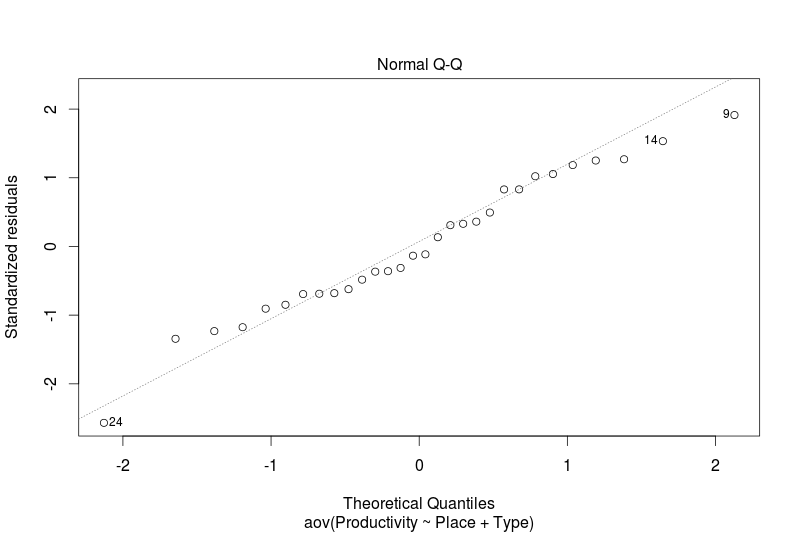
\includegraphics[scale=0.4]{qqplot.png}
  \caption{QQ-plot}
\end{figure}

Доверительные интервалы для урожайности и типа ячменя изображены на рис. 4.
По ним видно, что существенные отличия есть в парах типов ячменя T-S и T-M.
Не такое существенное различие есть в паре V-T.

Доверительные интервалы для урожайности и поля изображены на рис. 5.
По ним видно, что существенные отличия есть в парах полей W-UF, W-M, W-GR, W-D, W-C, M-GR, GR-C и D-C.

\section{Вывод}

Ячмень типа T более плодороден, чем ячмень типов S, M и V.

\begin{figure}[h]
  \centering
  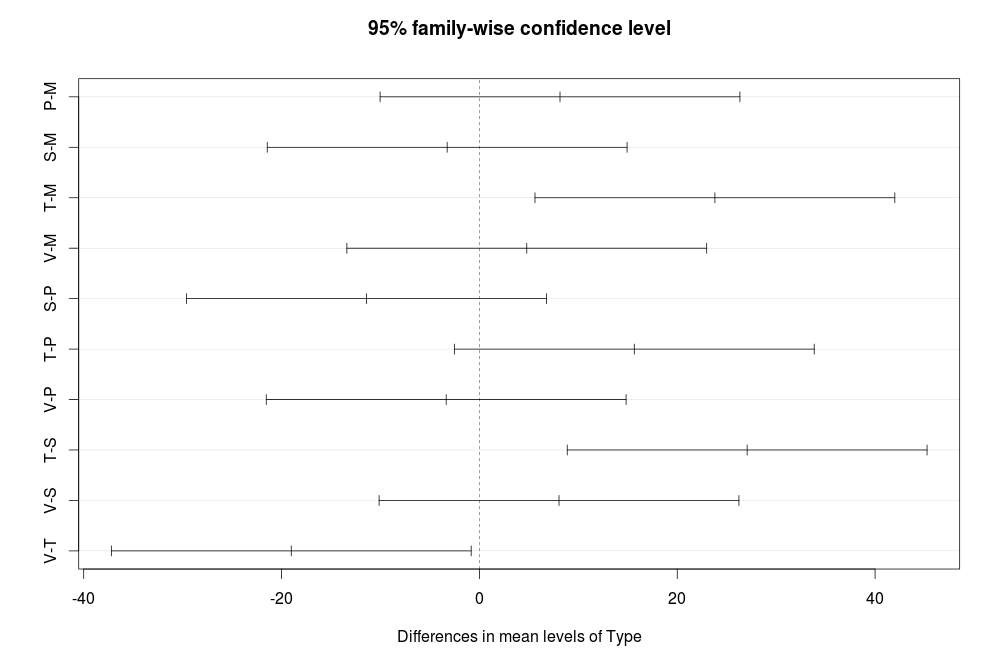
\includegraphics[scale=0.32]{ci_type.png}
  \caption{Доверительные интервалы для урожайности и типа ячменя}
\end{figure}

\begin{figure}[h]
  \centering
  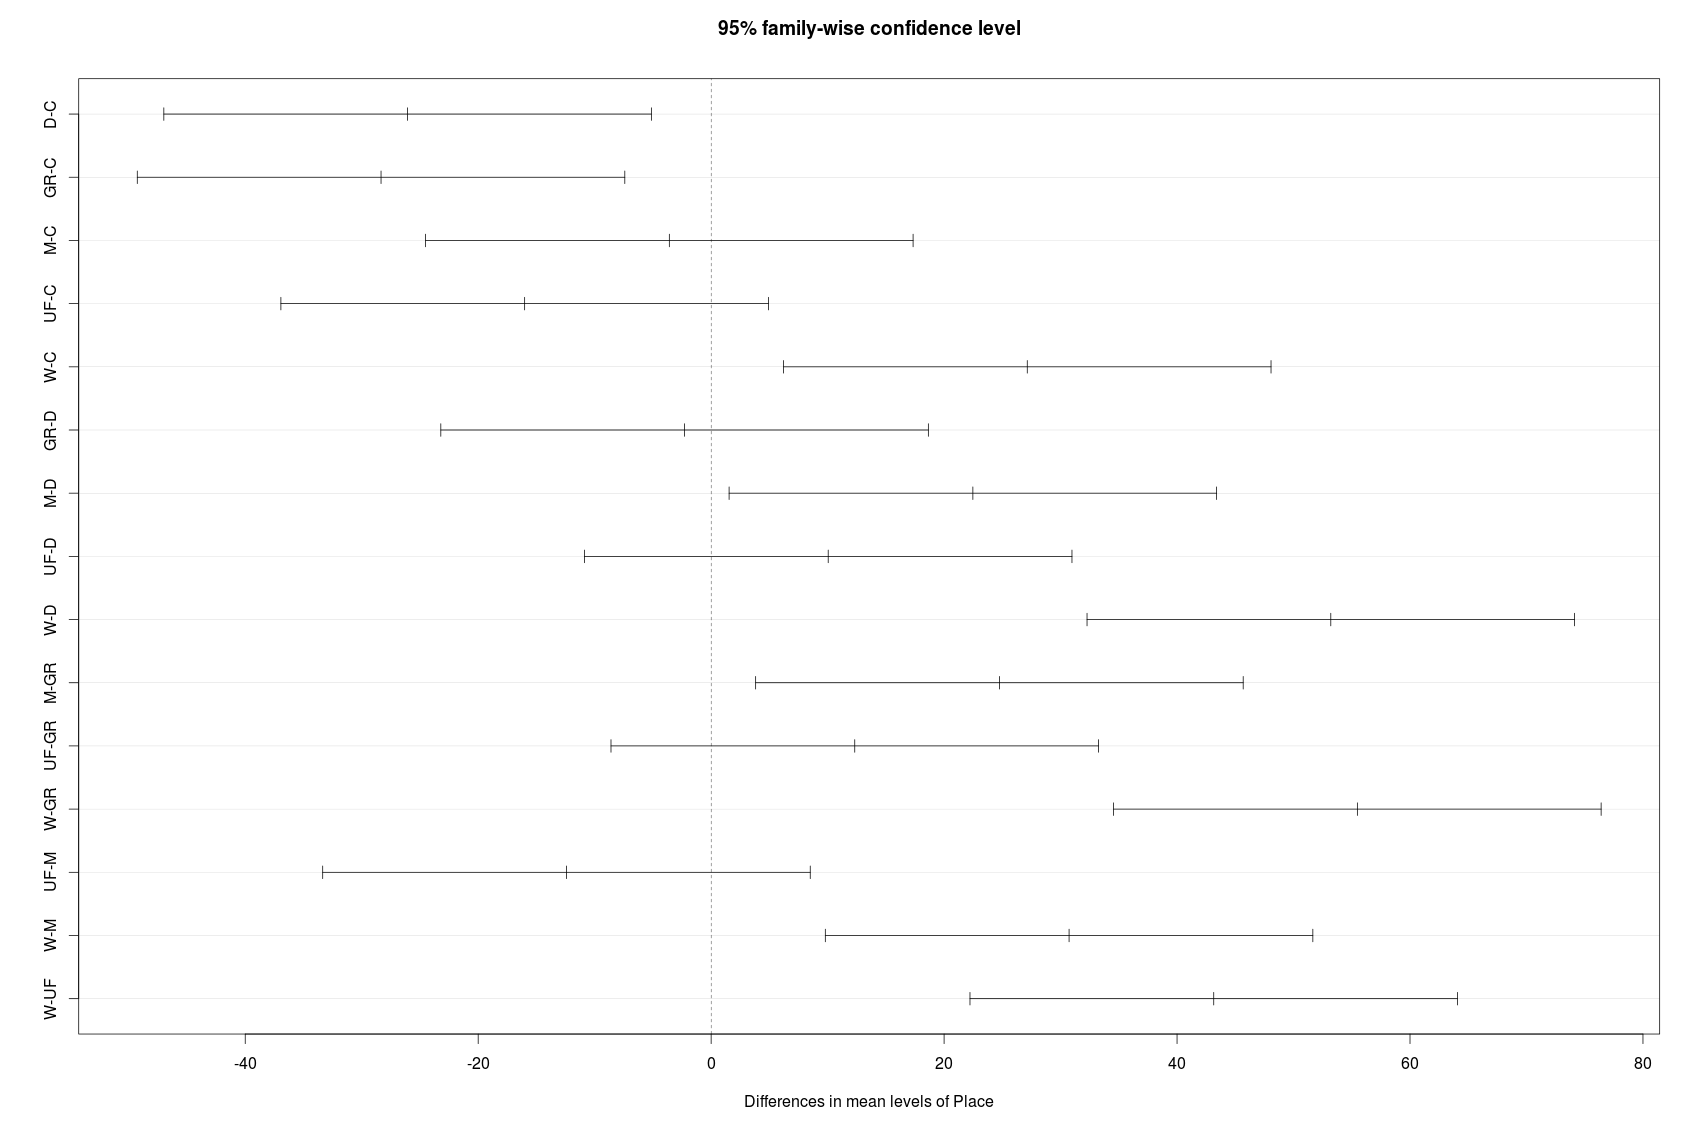
\includegraphics[scale=0.2]{ci_place.png}
  \caption{Доверительные интервалы для урожайности и поля}
\end{figure}

\end{document}
